%With increased precision of data, the calculations must also progress to higher accuracy, involving an increased number of diagrams with each 
%additional order, and this translates into computationally demanding 
%calculations even for the DIS processes. Such calculations 
%are too slow to be used iteratively in a fit.
%There are several methods available which allow fast PDF extractions.  
%Two such techniques
%are implemented into \fitter: the $k$-factor approximation from lower to higher order in theoretical precision and the fast grid techniques using interfaces to the 
%packages \texttt{fastNLO} \rm and \texttt{APPLGRID}. These techniques are briefly described below.  
%\\
More precise measurements
require theoretical predictions with equally improved accuracy in
order to maximize their impact in PDF fits.  Perturbative
calculations, however, get more and more involved with increasing
number of Feynman diagrams at each higher order. 
Nowadays even the most advanced perturbative techniques in
combination with recent computing hardware do not lead to sufficiently
small turn-around times. The direct inclusion of computationally
demanding higher-order calculations into iterative fits therefore is
not possible. Relying on the fact that a full repetition of the
perturbative calculation for arbitrary changes in input parameters is
not necessary at each iteration step, two methods have been developed
to resolve this problem: the techniques of $k$-factors and
\emph{fast grids}. Both are available in \fitter and described in the following.

\begin{description}
\item{\bf$k$-factor technique:}

  $k$-factors are defined as the ratio of the prediction of a
  higher-order (slow) pQCD calculation to a lower-order (fast)
  calculation. Because the $k$-factors depend on the phase space
  probed by the measurement they have to be stored into a table in
  dependence of the relevant kinematic variables. Before the start of
  a fitting procedure the table of $k$-factors has to be computed once
  for a given PDF with the time consuming higher-order code. In
  subsequent iteration steps the theory prediction is derived from the
  fast lower-order calculation multiplied by the pre-tabulated
  $k$-factors.

  However, this procedure neglects the fact that the $k$-factors are
  process dependent and, 
%  and are, for example, different for dijet
%  production from quark-quark or gluon-gluon initial states. 
  as a consequence, they have to be re-evaluated
  for the newly determined PDF at the end of the fit in order to check
  for any changes. Usually, the fit is repeated until input and output
  $k$-factors have converged. In summary, this technique avoids to
  iterate the higher-order calculation at each step, but still
  requires a couple of repetitions depending on the analysis.


\begin{itemize}
%\item For the DIS process, the heavy flavour schemes provide accurate but computationally slow calculations. 
%In \fitter ``FAST'' schemes were implemented 
%such that the $k$-factors used can be
%the ratio between same order calculations but massive versus massless
%i.e. NLO (ACOT)/NLO (ZM-VFNS), or 
%the ratio between NLO (massive)/LO (massless).
%The $k$-factors are only calculated for the PDF parameters at the first 
%fit iteration
% and hence, the FAST heavy flavour schemes should only be used 
%for quick checks and the full scheme is recommended.
%%%%
%The method was employed in the QCD fits to the HERA data when ACOT scheme was used as a cross check of the central results \cite{h1zeus:2009wt}, as shown in Fig.~\ref{fig:acotrt}.
%
  \item In DIS, the special case occurs of accurate but
    computationally slow calculations of the heavy flavour schemes.
    For this purpose, ``FAST'' heavy flavour schemes are implemented
    in \fitter with $k$-factors defined as the ratio of
    calculations at the same perturbative order but for massive vs.\
    massless quarks, e.g.\ NLO (massive)/NLO (massless).
    In the \fitter
    implementation, these $k$-factors are calculated only for the
    starting PDF and hence, the ``FAST'' heavy flavour schemes should
    only be used for quick checks, i.e. full heavy flavour schemes
    are recommended
    %and it is recommended to apply the full heavy flavour schemes 
    (with an exception of ACOT case 
    where, due to long computation time, the $k$-factors are used in 
    the default settings).

    This ``FAST'' method was employed in the QCD fits to the HERA data
    shown in Fig.~\ref{fig:acotrt}. In this case, the ACOT scheme was
    used as a cross check of the central results~\cite{h1zeus:2009wt}.



\begin{figure}[!ht]
   \centering
   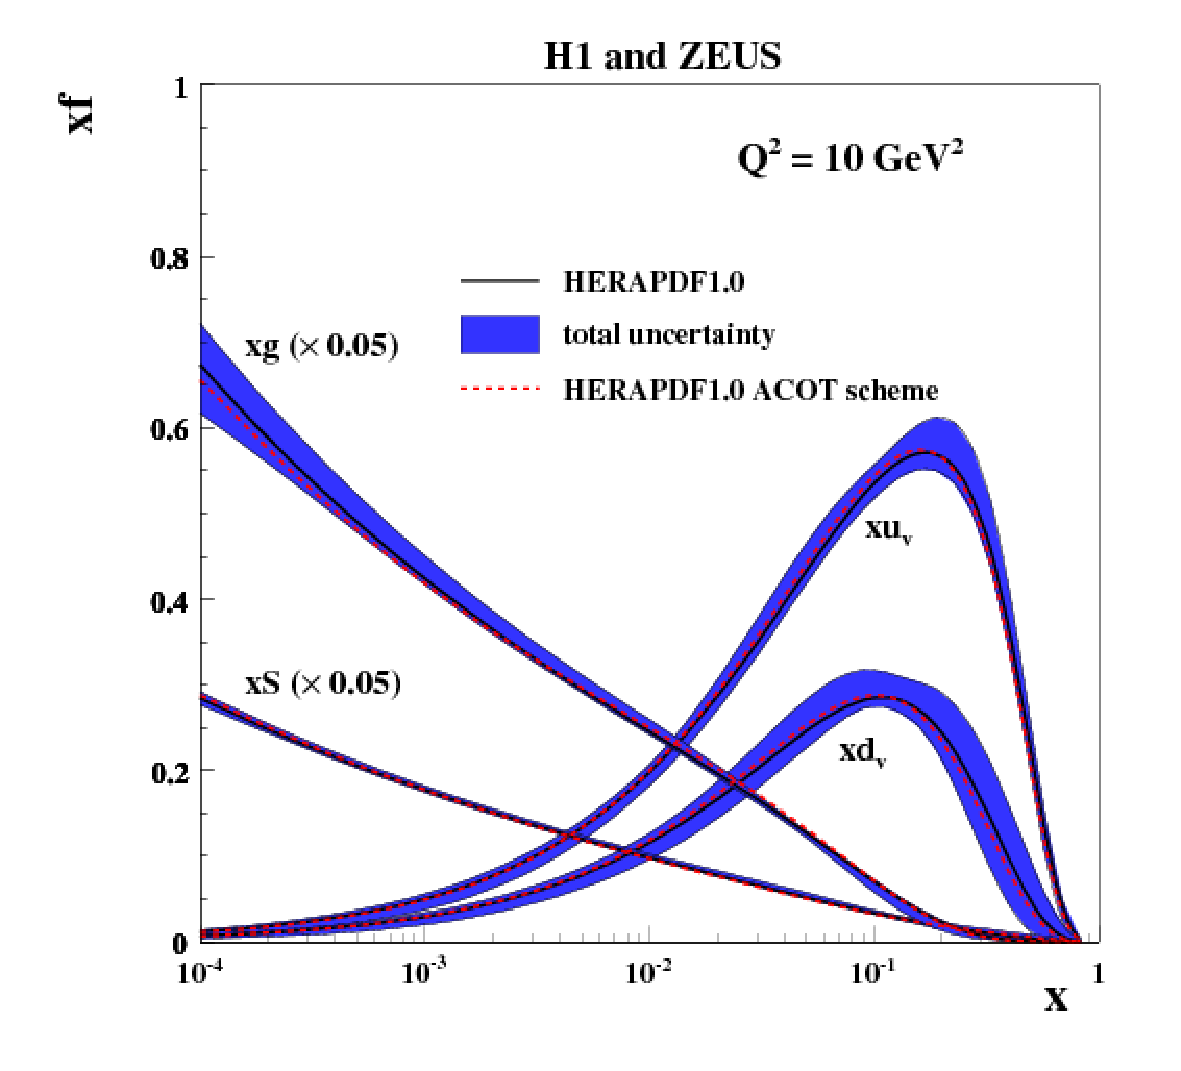
\includegraphics[width=8cm]{heraacot.pdf}
   \caption{Summary plots of valence, total sea (scaled) and gluon (scaled) densities with their total model uncertainties at the scale of $Q^2=10 \ \GeV^2$ obtained using the ACOT scheme with the $k$-factor method (red) compared to the HERAPDF1.0 PDF set at NLO using the TR' scheme.}
 \label{fig:acotrt}
\end{figure}



\item 
In the case of the DY processes the LO calculation described in section~\ref{dysection}
is such that the PDFs can be factorised, allowing high speed calculations when 
performing QCD fits over lepton rapidity data. In this case
the factorised part of the expression which is independent of PDFs can be
calculated only once for all minimisation iterations.
The leading order code in \fitter package implements this 
optimisation and uses fast convolution routines provided by
\qcdnum. Currently the full width LO calculations are optimised 
for lepton pseudorapidity and boson rapidity distributions with the
possibility to apply lepton \(p_{\perp}\) cuts.
%making this procedure flexible to describe data.
This flexibility allows the calculations to be performed within the phase space
corresponding to the available measurement.
%The calculated leading order cross sections are multiplied by
%NLO or NNLO k-factors provided for corresponding data distributions.
The calculated LO cross sections are multiplied by
$k$-factors to obtain predictions at NLO.

\end{itemize}

%or NNLO precision.
%%%%
%\subsubsection{APPLGRID}
%\vspace{0.1cm}

\vspace*{0.25cm}
\item \bf {Fast Grid Techniques:} \rm


\begin{itemize}
    \item The \applgrid~\cite{Carli:2010rw} package allows the fast computation 
of NLO cross sections for particular processes for arbitrary sets of 
proton parton distribution functions. The package implements
calculations of DY production as well as jet production in $pp(\bar p)$
collisions and DIS processes. 

The approach is based on storing the perturbative coefficients
of NLO QCD calculations of final-state observables measured
at hadron colliders in look-up tables. The PDFs and the 
strong couplings are included during the final calculations,
e.g. during PDF fitting. The method allows 
variation of factorisation and renormalisation scales in
calculations.

The look-up tables (grids) can be generated with modified versions
of the \texttt{MCFM} parton level generator for DY~\cite{Campbell:1999ah,Campbell:2000je,Campbell:2010ff} 
or \nlojetpp~\cite{Nagy:1998bb,Nagy:2001fj} code for NLO jet production.
The model input parameters are pre-set as usual for \texttt{MCFM}, 
while binning and definitions of the
cross section observables are set in the \applgrid code.
%as distributed with the full version of APPLGRID package.
% NLO calculations
%for the current analysis are performed with the help of APPLGRID
%generated grids based on MCFM calculations. 
%
%APPLGRID supports an interface to the MCFM parton level generators,
%hence model input parameters such as electroweak parameters
%are in fact pre-set following the MCFM input steering card, while
%binning and definitions of the observables for which the
%differential cross sections are needed are set in the 
%APPLGRID code. 
%The grid parameters \(x_1, x_2\) and \(Q^2\) binning
The grid parameters, \(Q^2\) binning
and interpolation orders are also defined in the code.

\applgrid constructs the grid tables in two 
steps: {\it (i)} exploration of the phase space in order
to optimize the memory storage and {\it (ii)} actual grid
construction in the phase space corresponding to the 
requested observables.
The NLO cross sections are restored from the grids
using externally provided PDFs, $\as$, factorization and 
renormalization scales. For NNLO predictions $k$-factors can be applied.

This method was used by the ATLAS collaboration in determining the strange 
quark density of the proton from $W$ and $Z$ cross sections 
together with HERA inclusive DIS data~\cite{atlas:strange}. 
An illustration of PDFs extracted in~\cite{atlas:strange} using \applgrid method 
and $k$-factors to correct from NLO to NNLO is shown 
in Fig.~\ref{fig:atlas} togehter with the comparison to the global PDF sets 
CT10~\cite{CT10pdf} and NNPDF2.1~\cite{NNPDFpdf}.

\begin{figure}[!ht]
   \centering
   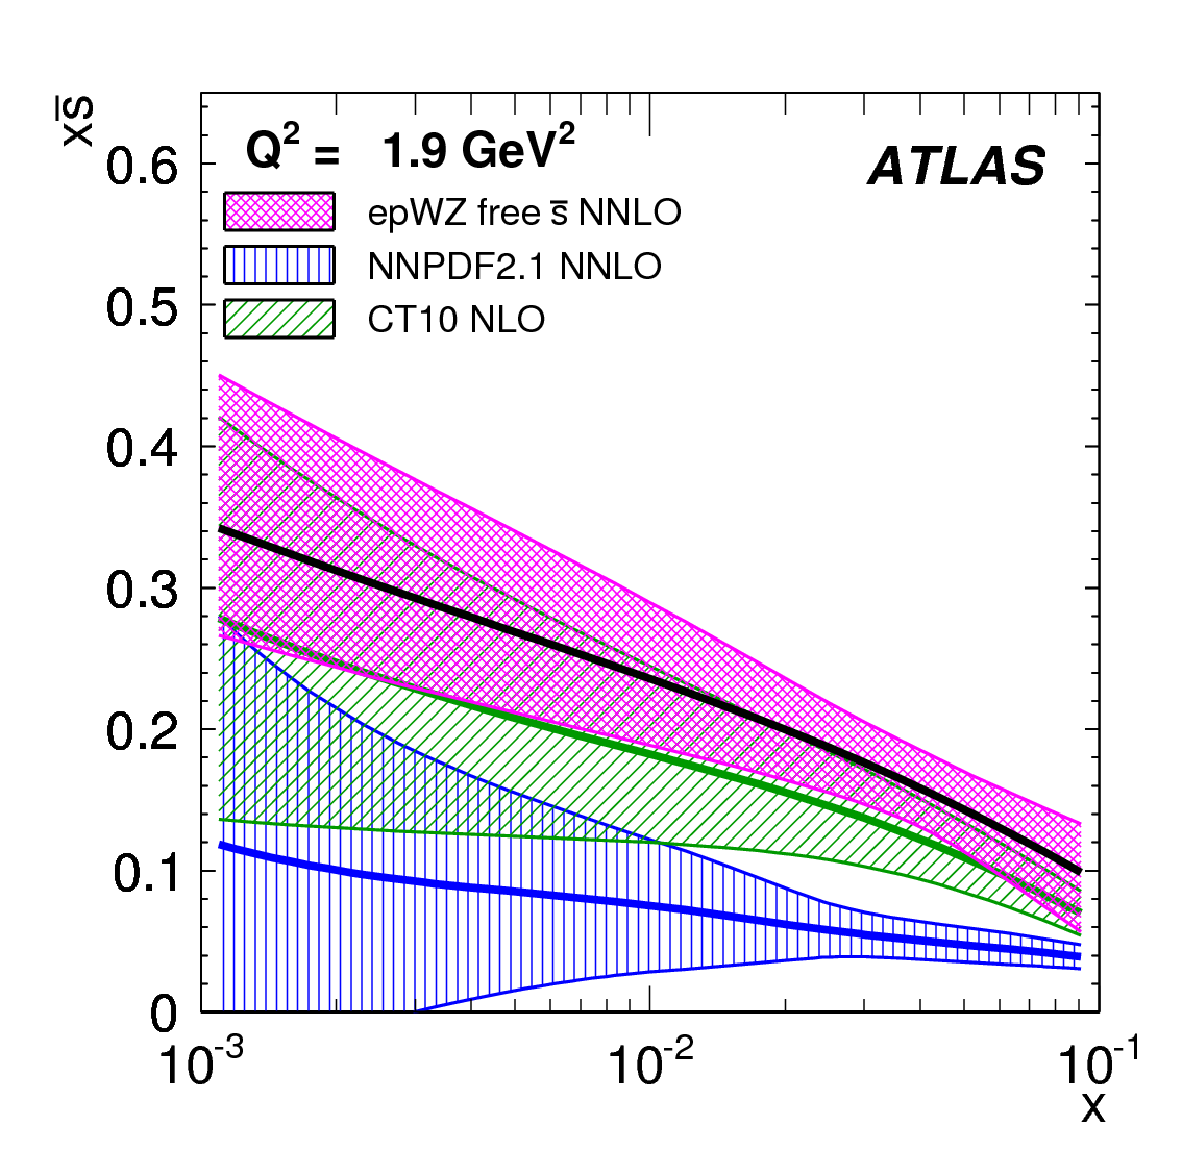
\includegraphics[width=8cm]{atlas.pdf}
   \caption{The strange anti-quark density versus $x$ for the ATLAS epWZ free sbar NNLO fit (magenta band) compared to predictions from NNPDF2.1 (blue hatched) and CT10 (green hatched) at $Q^2= 1.9 \ \GeV^2$.}
 \label{fig:atlas}
\end{figure}


\item
    The \fastnlo project~\cite{Kluge:2006xs,Wobisch:2011ij,Britzger:2012bs}
%enables the inclusion of jet data in PDF and $\alpha_s$ fits.
uses multi-dimensional interpolation
techniques to convert the convolutions of perturbative 
coefficients with parton distribution functions and 
the strong coupling into simple products.
%Although the concept is process independent, 
The perturbative 
coefficients are calculated by the \nlojetpp
program~\cite{Nagy:1998bb} where, 
in addition to the jet production processes available in \texttt{MCFM},
calculations for jet-production
in DIS~\cite{Nagy:2001xb} are available as well as calculations for 
hadron-hadron 
collisions~\cite{Nagy:2003tz,Nagy:2001fj} which include
 threshold-corrections 
at $\mathcal{O}$(NNLO) for inclusive jet cross 
sections~\cite{Kidonakis:2000gi}.

The  \fastnlo  libraries are included in the \fitter package.
%and no further requirements or compilation options
%are needed.
In order to include a new measurement into the PDF fit,
the \fastnlo tables have to be specified. These tables include all
necessary information about the perturbative coefficients and the
calculated process for all bins of a certain dataset. 
%Tables for almost all published jet measurements
%are available through the project website \\ {\tt http://fastnlo.hepforge.org}.
%
%Features of the fastNLO concept are the very quick convolution of the
%perturbative coefficients with the PDFs, of
%$\mathcal{O}(100 ms)$, and the very high accuracy
%of the interpolation procedure. 
The \fastnlo tables were originally calculated
for multiple factors of the factorization scale, 
and a renormalization scale factor could be chosen freely.
More recently, some of the \fastnlo tables allow for 
%already involve a scale-independent
%concept~\cite{Britzger:2012bs}, which allows for 
the free choice~\cite{Britzger:2012bs} of the renormalization and the factorization
scale as a function of two pre-defined observables.
The evaluation of the strong coupling constant, which enters
the cross section calculation, is taken consistently from the 
\qcdnum evolution code.

The \fastnlo methodology was used in the recent CMS analysis with \fitter where the impact
on the extraction of the PDFs from the inclusive jet cross section was investigated~\cite{cms:jets}. 
The impact of the gluon density of CMS inclusive jet data is illustrated in Fig.~\ref{fig:cmsjet}.
\begin{figure}[!ht]
   \centering
   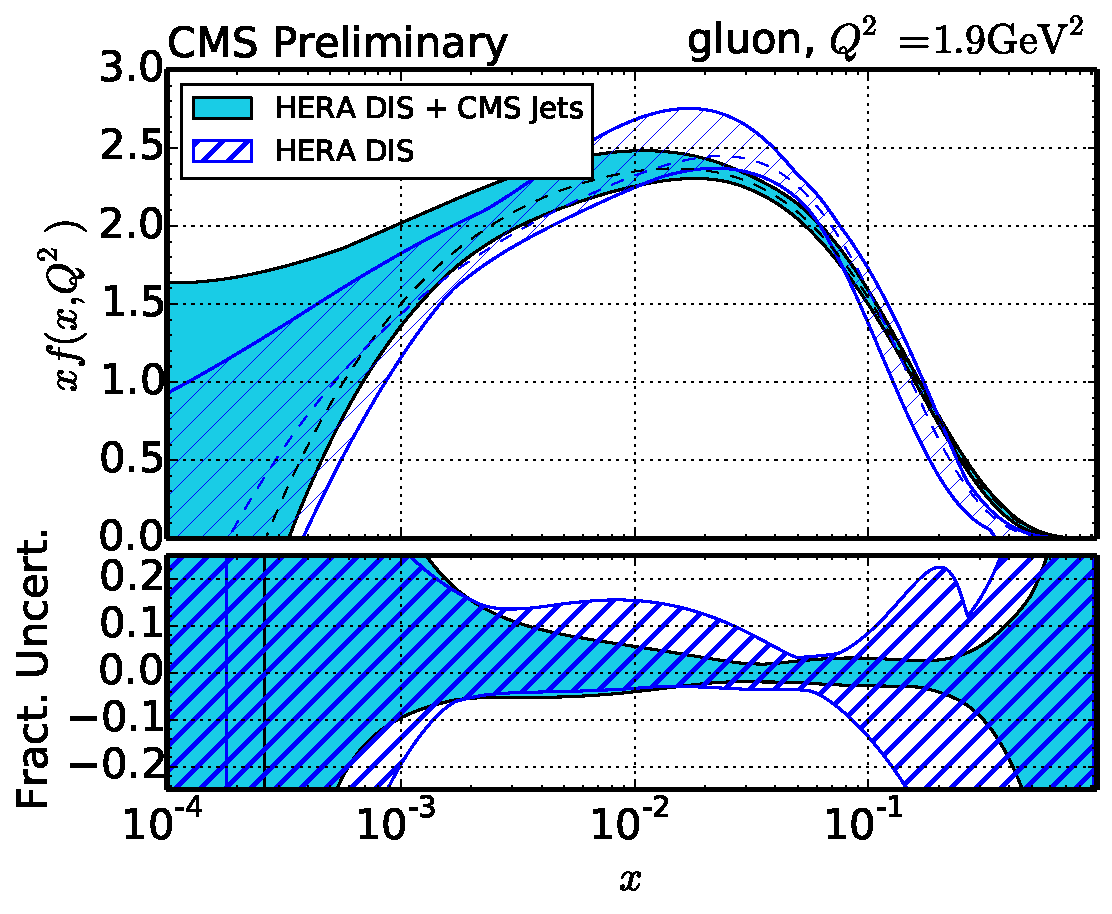
\includegraphics[width=8cm]{CMSjets.pdf}
   \caption{The gluon density as a function of $x$ as derived from HERA inclusive DIS data 
            alone (blue hatched) and in combination with CMS inclusive jet data from 2011 (cyan)
            where bands represent the total uncertainty of the PDFs. 
            The PDFs are shown at the starting scale $Q^2= 1.9 \GeV^2$.}
 \label{fig:cmsjet}
\end{figure}


\end{itemize}

\end{description}

